\chapter{Research And Approach}\label{ch:approach}
In this chapter we will cover the process of building the desired syntax of our language, and research into the domain.

The end goal of this chapter is to have ``working'' scripts for selected use cases.
The following chapter will then cover implementing the compilation of these scripts.


\section{Technologies}
In this section we will cover the technologies that will be involved in the final product.

\subsubsection{Language Considerations}
Before creating any code we have two language considerations to make.

The first consideration is the language to use for the compiler;
A good compiler tool is sufficiently portable that it is not difficult to use on any type of machine, historically this
has always been an issue, as Operating Systems and computer architecture have a wide variety - therefore the language
we use must be capable of creating executables for such a wide variety of systems.
In addition, as development time is significant, we should choose a language that provides sufficient tooling to
minimise unnecessary development time.

Our choice of compiler language is C#, due to its wide system compatibility and support of the~\cite{ANTLR} which we
will explore later.

Next we have to decide what language to compile to, which entails similar considerations as the user will want an
executable that requires minimal to no tweaking.
For this decision we have taken a slightly different approach - in order to fully leverage the language that we compile
to, we plan to support code injection - for this to remain convenient it's better to choose a language that more closely
resembles the one we're translating from.

In this train of thought, we have decided to compile to python, as it is a similarly high level language to the one
we are designing.

\subsubsection{Compiler Tools}\label{subsubsec:compilertools}
Our choice for compiler tooling follows a similar logic to most development tools, we would like ease of use, while
maintaining support for more complex functionality.

The main decision that had to be made was between ANTLR and leveraging the toolkit that intellij
provides~\cite{IntellijLanguage}.
After choosing ANTLR, we reasoned that we could take advantage of the parse tree that ANTLR creates for both debugging
and traversal properties - as ANTLR creates an easily readable image displaying how the grammar operates.
Furthermore, ANTLR introduces with it the listener pattern~\cite[p18]{ANTLRReference}

The document describing the syntax and semantics of a language is referred to as a ``grammar''\cite{Grammars}, both
ANTLR and the intellij plugin are based on Extended Backus-Naur Form (EBNF), they also both include a feature for
regex injection - allowing more well-formed rules to be written using fewer lines of code.

\subsubsection{Language Tools}
For the purpose of having usable output, we have decided to visualise the graphs we build.
The tool we'll be using for this purpose is GraphViz\cite{GraphViz} - which takes advantage of standardised grammar
called the DOT language, that can be used to consistently generate the same image.
Graphviz has a python library, so we can easily incorporate it into the print statements we define.


\section{Syntax}\label{sec:syntax}
The most visible part of any language is its syntax.
Each of us has a different background in terms of programming experience and preferences.
Inadvertently this will introduce some bias in our decision-making, but our distinct preferences
should counteract each others' biases.

Moreover, basing our language on existing languages may be somewhat counterproductive.
On one hand, creating a language that offers some familiarity to experienced programmers is a benefit,
however, following existing conventions defeats the purpose of the project i.e.: creating a language designed around graphs.
This was the mindset we had when setting out to design the syntax of Lattice.

Before getting into the concrete decisions we made, it is important to elaborate on our process, and the questions
we posed to ourselves.

\subsection{Verbosity and Obscurity}\label{subsec:syntax_verbostiy_and_obscurity}
Verbosity and obscurity are two opposing characteristics when designing language.
We could design a language that
relies heavily on English, making it accessible for new developers.
However, incessant verbosity may slow down experienced users when developing code.

Inversely, relying on obscure and arbitrary (but shorter) notations will
steepen the learning curve and may reduce readability.

In general, if we imagine the problem as a curve between verbosity and obscurity, we have fallen closer to
obscure choices with our decisions.
The reason for this is that we had to come up with various, previously
non-existent operators, and built-in functions working on a graph.
We, as a group also have a subjective preference for shorter, more obscure notation, the idea being that
after the initial learning period, its benefits offset the drawbacks.


\subsection{Ambiguity in Ownership and Operators}\label{subsec:syntax_ambigoutiy_in_ownership_and_operators}
The main problem we immediately encountered was ambiguity.
Consider the following questions:

\begin{enumerate}
    \item Can a node be added to two graphs?
    \item Can an edge exist between nodes belonging to different graphs?
\end{enumerate}

Suppose the answers are yes to both questions, as we wish to create a flexible language.
The desired operators are to be detailed later, but one of them is an operator that returns a list of edges belonging to a node.

Consider a simple program that creates the structure shown on figure~\ref{fig:syntax_ambigous}.
If within that structure, we were to apply said operator on \lstinline{shared_node} that belongs to two graphs and has edges within both graphs,
the operator would work ambiguously.
The operator may return any of the following:

\begin{enumerate}
    \item The operator returns the edges defined within graph 1
    \item The operator returns the edges defined within graph 2
    \item The operator returns the edges belonging to both graphs.
\end{enumerate}

\begin{figure}[H]
    \centering
    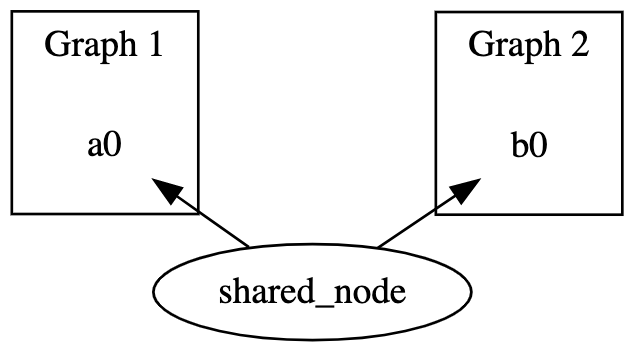
\includegraphics[width=6cm]{figures/syntax_section/syntax_ambigous}
    \caption{An example of a graph displaying a potentially ambigous situation.}
    \label{fig:syntax_ambigous}
\end{figure}



Each of these behaviours is equally valid.
Moreover, depending on the context, the user may wish to use any one of them.
The obvious solution is to split the operator into three distinct operators or expand it with a graph parameter.
However, if we consider that this is a single example of the problem, and the actual issue is systematic,
increasing the operator count or complexity only degrades the readability of the code and introduces the potential for bugs
both when using the language and when implementing it.

Our proposed solution is therefore to treat graphs as contexts.
Every operation performed inside a context, explicitly belongs to that graph.
This approach forbids the previously stated questions.
However, we intend to make the graphs nestable, while a node cannot belong to two distinct graphs,
it may belong to both of them in the context of a parent graph.
Therefore, if we want to get a list of the edges belonging to graph 1, connected to the node, we may perform the
operation in the context of graph 1.
If we want to return all the edges, we may perform it in the context of the parent graph.

\subsection{Assignment and Types}\label{subsec:syntax_assignment_and_types}
Before introducing the core of Lattice - graphs, it is important to explicitly state basic functionality,
such as variables and assignments.
We have chosen to explicitly state the type of a variable at declaration,
following the form of \lstinline{type var_name = value}.
THe example listing~\ref{lst:syntax_basic_var_dec} shows how variables are declared in Lattice.

We also settled on a set of primitive types we intend to implement, namely:
\begin{itemize}
    \item Integer - (int)
    \item String - (str)
    \item Boolean - (bool)
    \item Float - (float)
\end{itemize}

\begin{lstlisting}[caption={Basic variable declaration.},captionpos=b,label={lst:syntax_basic_var_dec}]
    int a = 1;
    str text = "text";
    bool boolExpr = true;
    float half = 0.5;
\end{lstlisting}



\subsection{Branching}\label{subsec:syntax_branching}
We have decided to implement the simplest form of branching, a simple if-else block.
While additional branching options are nice to have, such as else-if (also known as elif) or switch statements, their
expressive power is the as same if-else.

The syntax will be C-like as shown in listing~\ref{lst:syntax_basic_if_else}
\begin{lstlisting}[caption={Simple branching example.},captionpos=b,label={lst:syntax_basic_if_else}]
    bool foo = true;
    if(foo) {
        print "foo"
    }
    else {
        print "bar"
    }
\end{lstlisting}

\subsection{Graphs}\label{subsec:syntax_graphs}
Graphs are the concept around which the whole language is built around.
Therefore, the definition of graphs
must be simple and concise.
The notation must also allow the usage of contexts.
Ultimately we ended up with a syntactic solution we believe is simple and easy to read.
Below is an excerpt for
defining a graph with two nodes.

\begin{lstlisting}[caption={Graph declaration.}, captionpos=b, label={lst:syntax_basic_graph_definition}]
    graph g1 {
        ref int a = 5;
        ref str b = "foo";
    }
\end{lstlisting}

\begin{figure}[H]
    \centering
    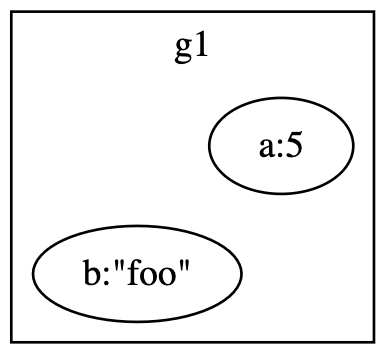
\includegraphics[width=6cm]{figures/syntax_section/syntax_simple_graph}
    \caption{A simple graph generated by~\ref{lst:syntax_basic_graph_definition}}
    \label{fig:syntax_basic_graph}
\end{figure}

Listing~\ref{lst:syntax_basic_graph_definition} generates the graph shown on figure~\ref{fig:syntax_basic_graph}

The graph keyword, when binding the graph may seem unnecessary.
However, a potential extension we have considered was inheritance.
So in the future, one may define a specific type of graph
e.g.\ Tree or LinkedList, which conceptually are just restricted graphs.

The context of graphs may be reopened as well.
So the snippet shown on listing~\ref{lst:syntax_basic_graph_definition}
may be extended with a third node (listing~\ref{lst:syntax_basic_graph_defintion_extended})
even after the declaration of the node - generating figure~\ref{fig:syntax_basic_graph_extended}

\begin{lstlisting}[caption={Extending a graph.},captionpos=b,label={lst:syntax_basic_graph_defintion_extended}]
    graph g1 {
        ref int a = 5;
        ref str b = "foo";
    }
    print "outside of the g1 context";
    g1 {
        ref bool c = false;
    }
\end{lstlisting}

\begin{figure}[H]
    \centering
    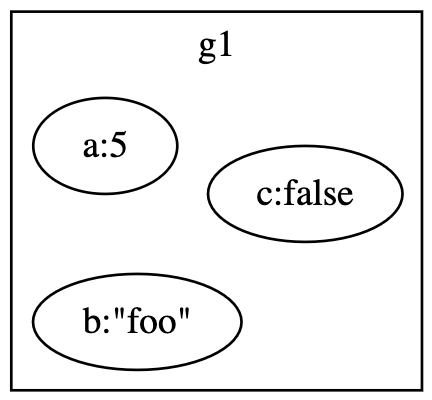
\includegraphics[width=6cm]{figures/syntax_section/syntax_basic_graph_extended}
    \caption{A graph extended by reopening the context, generated by listing~\ref{lst:syntax_basic_graph_defintion_extended}}
    \label{fig:syntax_basic_graph_extended}
\end{figure}

To create sub-graphs, one may open a sub-context inside an existing graph.
The child graph will not implicitly inherit the parent nodes, but they must be explicitly referenced or cloned.
This allows the user to create proper sub-graphs.
Listing~\ref{lst:syntax_basic_subgraph} shows the code for creating such sub-graphs, resulting in figure~\ref{fig:syntax_basic_subgraph}

\begin{lstlisting}[caption={Creating a sub-graph g2 in the context of g1},captionpos=b, label={lst:syntax_basic_subgraph}]
    graph g1 {
        ref int a = 5;
        ref str b = "foo";

        g2 {
            ref a;
        }
    }
\end{lstlisting}
\begin{figure}[H]
    \centering
    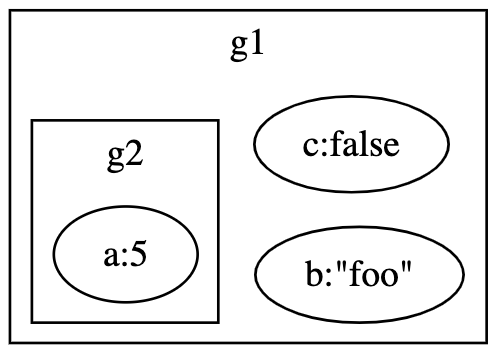
\includegraphics[width=6cm]{figures/syntax_section/syntax_basic_subgraph}
    \caption{A graph extended by reopening the context, generated by~\ref{lst:syntax_basic_subgraph}.}
    \label{fig:syntax_basic_subgraph}
\end{figure}

\subsection{Nodes}\label{subsec:syntax_nodes}
Similar to graphs, nodes ought to be first-class citizens in Lattice.
Initially, we experimented with the
idea of having every declared variable act as implicit nodes in the graph.
However, when writing example programs it quickly became a nuisance.
Any program with any degree of complexity will inevitably use \("\)helper\("\) variables.
These variables may be simple things such as loop iterators, or the result of boolean expressions.
Programmers will not necessarily intend to include these variables as parts of the graphs.

Therefore, variables intended to be used as nodes will have to be prefixed either by the \lstinline{ref}
or the \lstinline{clone} keyword.

The keyword naming is self-explanatory.
\lstinline{Ref} introduces the node in the graph by its reference, such that if
the node is changed in a different context, its value will change in every graph.
Contrary to that, when cloning, the node's data will be copied over to the graph with its current value.

Listing~\ref{lst:syntax_ref_clone_difference_node} and figure~\ref{fig:syntax_ref_vs_clone} show the difference between ref and clone.

\begin{lstlisting}[caption={Example code, showcasing the difference between ref and clone.},captionpos=b,label={lst:syntax_ref_clone_difference_node}]
    int a = 5;
    int b = 6;

    graph g1 {
        ref a;
        clone b;
    }
    a = 10;
    b = 12;
\end{lstlisting}
\begin{figure}[H]
    \centering
    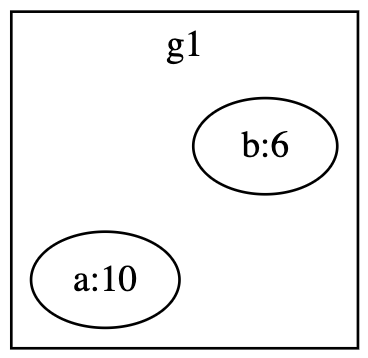
\includegraphics[width=6cm]{figures/syntax_section/syntax_ref_vs_clone}
    \caption{A graph showcasing the difference between \lstinline{ref} and \lstinline{clone}, generated by~\ref{lst:syntax_ref_clone_difference_node}.}
    \label{fig:syntax_ref_vs_clone}
\end{figure}

These keywords may also be applied to graphs when sub-graphing behaviour is required.
In this case the difference in the behaviour of \lstinline{ref} and \lstinline{clone} is the same.

\begin{lstlisting}[caption={Ref and clone with graphs.},captionpos=b, label={lst:syntax_ref_clone_difference_graph}]

    graph g1 {
        ref int a = 5;
    }
    graph g2 {
        ref int b = 6;
    }
    graph g1ug2 {
        ref g1;
        clone g2;
    }
    g1 {
        ref int a = 10;
    }
    g2 {
        ref int b = 12;
    }
}
\end{lstlisting}
\begin{figure}[H]
    \centering
    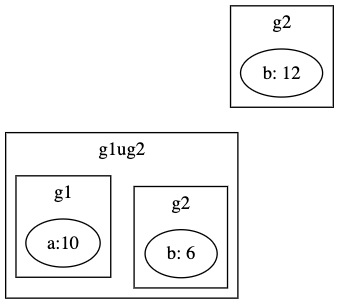
\includegraphics[width=6cm]{figures/syntax_section/syntax_ref_vs_clone_graphs}
    \caption{A graph extended by reopening the context, generated by listing~\ref{lst:syntax_ref_clone_difference_graph}.}
    \label{fig:syntax_ref_vs_clone_with_graphs}
\end{figure}

An interesting discovery we made during the development of mock code, it was easier to write unambiguous code
when the nodes were treated as immutable.
So listing~\ref{lst:syntax_immutability_valid} is a valid Lattice code, while listing~\ref{lst:syntax_immutability_invalid} is not.

\begin{lstlisting}[caption={Valid destruction and recreation of nodes.},captionpos=b,label={lst:syntax_immutability_valid}]
    graph g1 {
        ref int a = 5;
    }
    g1 {
        ref int a = 6;
    }
\end{lstlisting}

\begin{lstlisting}[caption={Code violating the immutability of nodes.},captionpos=b,label={lst:syntax_immutability_invalid}]
    graph g1 {
        ref int a = 5;
    }
    g1 {
        a = 6;
    }
\end{lstlisting}


\subsection{Operators}\label{subsec:syntax_operators}
As mentioned before, we introduce some obscure notation in our design.
The reasoning is that we want to support operations that are generally either not supported in other languages
or only supported via external libraries that are dependent on the language's own syntax.

While we are not going to change the operator for adding two integers together (\lstinline{int1 + int2}),
we are going to create our own arbitrary notation for graph operations since it is a new territory.

For example, if we were to build an edge between two nodes,
Lattice will provide the following built-in operators to do so:

\begin{itemize}
    \item \lstinline{node1 <-"label1",5-> node2}
    \item \lstinline{node1 |-"label2",0.5-> node2}
\end{itemize}

Which will generate the graph shown on figure~\ref{fig:relation_basic_operator}
\begin{figure}[H]
    \centering
    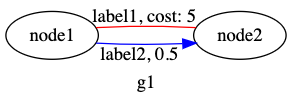
\includegraphics[width=6cm]{figures/syntax_section/syntax_rel_basic}
    \caption{Example graph showcasing various edge operators.}
    \label{fig:relation_basic_operator}
\end{figure}


The first operator creates an undirected edge between \lstinline{node1} and \lstinline{node2}, with a label: \("\)label1\("\) and a cost of 5.
The second operator creates a directed edge between \lstinline{node1} and \lstinline{node2} where \lstinline{node1}
is the predecessor and \lstinline{node2} is the successor.
The labelling and cost behaviour are the same for the two operators.

In an ideal world, the label and cost parameters would be optional.
However, it is one the restrictions we made to reduce the scope of the project.

We also want to allow programmatic graph traversal.
The easiest way to achieve it is to introduce query operators, which may be used to move along the graph.

\begin{itemize}
    \item \lstinline{node1->?} returns all the directed edges where \lstinline{node1} is the predecessor.
    \item \lstinline{?->node1} returns all the directed edges where \lstinline{node1} is the successor.
    \item \lstinline{node1-|?} returns every undirected edge connected to \lstinline{node1}.
    \item \lstinline{rel1?} returns the successor node of \lstinline{rel1}.
    \item \lstinline{?rel1} returns the predecessor node of \lstinline{rel1}.
    \item \lstinline{?rel2?} returns a pair of nodes, assuming that \lstinline{rel1} is an undirected edge.
\end{itemize}

If the above operators were applied on the graph shown on figure~\ref{fig:syntax_query_operators_example_out}.
The following would be returned:

\begin{itemize}
    \item \lstinline{node1->?} returns \lstinline{node2}.
    \item \lstinline{?->node1} returns \lstinline{node3}.
    \item \lstinline{node1-|?} returns \lstinline{node2} and \lstinline{node4}.
    \item \lstinline{rel1?} returns \lstinline{node2}.
    \item \lstinline{?rel1} returns \lstinline{node1}.
    \item \lstinline{?rel2?} returns \lstinline{node1} and \lstinline{node4}.
\end{itemize}

\begin{figure}[H]
    \centering
    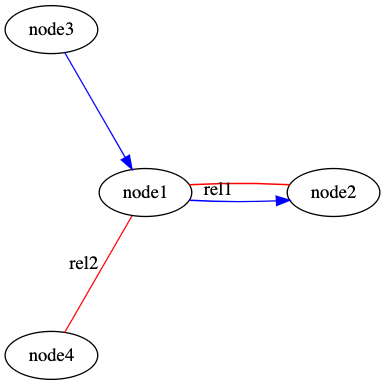
\includegraphics[width=6cm]{figures/syntax_section/syntax_query_operators}
    \caption{Example graph to show the usage of query operators.}
    \label{fig:syntax_query_operators_example_out}
\end{figure}

Besides the graph-specific operators, we include a suite of well-known basic operators.
Below is a categorized list of the operators we intend to implement:


\textbf{Boolean operators}
\begin{itemize}
    \item \lstinline{&&} - boolean \emph{and} operator.
    \item \lstinline{||} - boolean \emph{or} operator.
    \item \lstinline{!} - boolean \emph{negate} operator.
    \item \lstinline{==} - boolean \emph{equality} operator.
    \item \lstinline{!=} - boolean \emph{inequality} operator.
    \item \lstinline{<} - \emph{less than}.
\end{itemize}

\textbf{Numeric operators}
\begin{itemize}
    \item \lstinline{+} - \emph{addition}.
    \item \lstinline{-} - \emph{subtraction}.
    \item \lstinline{*} - \emph{multiplication}.
    \item \lstinline{/} - \emph{division}.
    \item \lstinline{%} - \emph{modulo}.
\end{itemize}

There are some well-known operators left out, such as \lstinline{<=} or \lstinline{>}.
Simply because while it is arduous to work around them, it is still possible to do so.
For example  \lstinline{int1 <= int2} may be expressed with:  \lstinline{int1 < int2 || int1==int2}.

\subsection{Edges}\label{subsec:syntax_edges}
The final, essential component for a language for graphs are edges.
In the previous section, their operators have been introduced,
they do, however, have to exist as standalone objects as well.
If they only exist within the operations, the power of the language is rather
limited.

Therefore, the above-mentioned operation node1 \lstinline{<-"label1",5-> node2}, returns a relationship object (a common, shared
type for directed and undirected edges).

So, the following would be valid code in Lattice: \lstinline{rel relationship = node1 <-"label1",5-> node2.}

Then, the developer may apply any of the relationship operations on r.

\subsection{Functions}\label{subsec:syntax_functions}
Functions are one of those well-known features that we believe improves Lattice significantly.
Having reusable blocks of code makes developing example code significantly easier.

In line with our implementation of \("\)if-else\("\) and \("\)while\("\) we have chosen to implement functions in a C-like manner.
They follow the basic structure of:

\lstinline|return_type function_name (arg_type arg_name) {statements; return return_value;}|

An example is shown in listing~\ref{lst:syntax_fmap_basic}

\subsection{Iteration and Enumeration}\label{subsec:syntax_iteration-and-enumeration}
Iteration, in the classical sense, is a simple, and well-explored concept.
We have chosen to only include while loops (listing~\ref{lst:syntax_syntax_while_basic})
in Lattice, as its expressive power, is equivalent to any other constructs, such as for, or foreach.

\begin{lstlisting}[caption={Simple while loop.},captionpos=b,label={lst:syntax_syntax_while_basic}]
    int iterator = 0;
    int max = 5;
    while(iterator < max) {
        print iterator;
    }
\end{lstlisting}


We find that while loops alone were insufficient to enumerate graphs.
Currently, there is no commonly accepted approach
for such operations.

Building a deterministic approach would be relatively easy.
We could, for example, apply the operations on the nodes in which
they were added.

However, we believe that the nature of the answers point to the fact that traditional approaches are insufficient for graph
enumeration.

Therefore, we have decided to try a functional approach.
Haskell's fmap fits our needs precisely.
It is a function that takes a function, and a custom data type as input, and applies the function to each member of
the entity.
The underlying implementation does not concern the user, nor is it apparent when it is used.

For example, in listing~\ref{lst:syntax_fmap_basic} we apply the function double to g1, and return a cloned instance
in the form of g2 (figure~\ref{fig:syntax_fmap_basic})

\begin{lstlisting}[caption={Simple fmap application on a graph.},captionpos=b,label={lst:syntax_fmap_basic}]
    graph g1 {
        ref int a = 5;
        ref int b = 6;
        ref int c = 7;

       a |-"ab",0-> b;
       b |-"bc",0-> c;
       c |-"ca",0-> a;
    }
    graph g2 = fmap double g1;

    int double(int node) {
        return node*2;
    }
\end{lstlisting}

\begin{figure}[H]
    \centering
    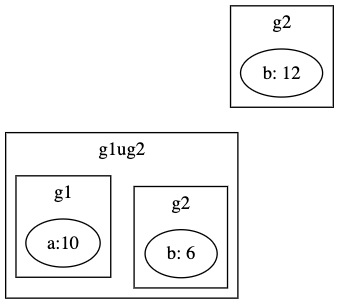
\includegraphics[width=6cm]{figures/syntax_section/syntax_ref_vs_clone_graphs}
    \caption{An application of fmap, where g2 is a clone of g1, with the double function applied. Generated by listing~\ref{lst:syntax_fmap_basic}.}
    \label{fig:syntax_fmap_basic}
\end{figure}


\subsection{Polymorphic Implications}\label{subsec:syntax_polymorphic_implications}
A notable omission from the previous sections was type behaviour.
If we were to consider that graphs do not have a single
type of node they accept like other strongly typed languages, such as C\# (\lstinline[language=C#]{List<int> intList = new List<int>();}),
and that fmap may be applied to any graphs, the code shown on~\ref{lst:syntax_invalid_fmap} is syntactically valid Lattice code.

\begin{lstlisting}[caption={Fmap applied on a graph that contains non-numeric values.},captionpos=b,label={lst:syntax_invalid_fmap}]
graph g {
    ref string a = "a";
    ref bool b = true;
    ref int c = 1;
}
graph g2 = fmap (+1) g;
\end{lstlisting}


This is the reason why we decided to have the nodes and functions strongly typed.
With strongly typed functions and nodes we may perform compile time type check, therefore while the syntax is valid,
it would be semantically invalid, and would result in a compiler error.


\subsection{Showcase: K-Sized Binary Tree}\label{subsec:syntax_showcase_k_sized_binary_tree}
Listing~\ref{lst:syntax_k_sized_tree} illustrates a potential program that may be written in Lattice.
It generates a binary tree of height K.
It does so by duplicating the previous instance of the tree, and connecting them by a new common root.

\begin{lstlisting}[caption={Lattice code generating a balanced binary tree of height K.},captionpos=b,label={lst:syntax_k_sized_tree}]
    int k = 5;
    int iterator = 0;

    str nodeVal = "node";

    str leftRoot;
    str rightRoot;


    graph left {}
    graph right {}
    graph bTree {
    }
    while(iterator < k) {
        if(iterator == 0) {
            bTree {
                clone nodeVal;
                str newRoot = nodeVal;
            }
        }
        else {
            bTree {
                clone left;
                clone right;

                newRoot |-"left",0-> leftRoot;
                newRoot |-"right",0-> rightRoot;

            }
        }
        left = clone bTree;
        right = clone bTree;
        left {
            str leftRoot = newRoot;
        }
        right {
            str rightRoot = newRoot;
        }
        iterator = iterator + 1;
    }
\end{lstlisting}

First, some helper variables are initialized, \lstinline{k} and \lstinline{iterator} will simply set the height of
the tree by controlling the while loop.
Then, \lstinline{nodeval} is just a simple placeholder value to fill the nodes.
The next two variables \lstinline{leftRoot} and \lstinline{rightRoot} will also act as temporary variables,
holding the value of the current root on each side.

The final step in the initialization is the declaration of three graphs: \lstinline{left}, \lstinline{right} and
\lstinline{bTree}, \lstinline{left} and \lstinline{right} will hold the previous iteration's tree, while bTree will hold
the final, output tree.

If it is the first iteration, then \lstinline{nodeval} is simple cloned into \lstinline{bTree}, making it a permanent node.
Also, a new variable is initialized: \lstinline{newRoot}, which will always hold the reference to the latest root node.
It is important to note, that this operation happened in the context of \lstinline{bTree}, therefore the variable may
be accessed later.

If it is not the first iteration, then, again in the context of \lstinline{bTree} the graphs \lstinline{left} and \lstinline{right}
are cloned making them subgraphs of \lstinline{bTree}.
Finally, in the else branch, a directed edge is constructed between the \lstinline{newRoot} and the roots of \lstinline{left} and \lstinline{right}
(\lstinline{leftRoot} and \lstinline{rightRoot}).
This is done using the directed edge operator \lstinline{|-"left",0->}.

Then, at the end of the loop, regardless if it is the first iteration or not, the values of \lstinline{left} and \lstinline{right}
are replaced with a clone of \lstinline{bTree}.
In the individual context of \lstinline{left} and \lstinline{right} the new roots are also set for each side.

Finally, the value of the \lstinline{iterator} is increased by one.






\section{Context-Free Grammar}\label{sec:grammar}
To specify some rules about how a program in Lattice should be composed, we have written the following context-free grammar, using Extended Backus-Naur form.
This grammar can then be used to build a parser and recognize valid Lattice programs and their structure.

\subsubsection*{Global composition of a program}

A program in Lattice would be a sequence of statements and function definitions.

\begin{align*}
    \mathit{Start} \rightarrow \{ \mathit{FunctionDef} \mid \mathit{Statement} \}
\end{align*}
\captionedgrammar{Description of the global structure of a program}

Statements can be variable declarations, variable assignments, graph manipulation (i.e.\ opening a graph context to do operations), print statements, blocks of code in an if-else control structure or a while loop, or a return statement.

\begin{align*}
    \omit $\mathit{Statement}$ \hfil& \rightarrow \mathit{VarDecl} \\
    & \mid \mathit{VarAssignOrGraphManip} \\
    & \mid \mathit{PrintStatement} \\
    & \mid \mathit{IfBlock} \\
    & \mid \mathit{WhileBlock} \\
    & \mid \mathit{ReturnStatement}
\end{align*}
\captionedgrammar{Description of the different kind of statements}

\subsubsection*{Variable declaration}

A variable is declared by writing its type followed by its name.
After the variable declarations the statement can end with a semicolon or there can be a value assigned to the variable or a graph context can be opened.

There need to be a global production rule for variable assignment and graph manipulation because both statements start with a variable identifier so having the rules be fully separated would mean that the grammar isn't LL(1).
Once the variable for which we are writing the statement is specified, the rest of the statement can either correspond to an assignment or to a block of code in a graph context.

\begin{align*}
    \omit $\mathit{VarDecl}$ \hfil& \rightarrow \mathit{Type} \: \text{varId} \: \mathit{VarDeclTail} \\
    \omit $\mathit{VarDeclTail}$ \hfil & \rightarrow \mathit{TailVarAssignOrGraphManip} \\
    & \mid \text{semicolon} \\
    \omit $\mathit{VarAssignOrGraphManip}$\hfil & \rightarrow \text{varId} \: \mathit{TailVarAssignOrGraphManip} \\
    \omit $\mathit{TailVarAssignOrGraphManip}$ & \rightarrow \mathit{TailVarAssign} \\
    & \mid  \mathit{TailGraphManip}\ \\
    \omit $\mathit{Type}$ \hfil & \rightarrow \text{typeString} \\
    & \mid \text{typeFloat} \\
    & \mid \text{typeBool} \\
    & \mid \text{typeInt}\\
    & \mid \text{typeGraph}
\end{align*}
\captionedgrammar{Rules for variable declaration}

\subsubsection*{Variable assignment and arithmetic expressions}
To assign a value to a variable, the variable name needs to be followed by the assignment operator and then the assigned value, which can be a string, a boolean value, an arithmetic expression with variables, numbers and function calls or simply a function call, a number or another variable.

\begin{align*}
    \omit $\mathit{TailVarAssign}$ \hfil & \rightarrow \text{opAssign} \: \mathit{AssignVal} \: \text{semicolon} \\
    \omit $\mathit{AssignVal}$ \hfil & \rightarrow \text{string} \\
    & \mid \mathit{Expr} \\
    & \mid \mathit{BoolVal}\\
    \omit $\mathit{Expr}$ \hfil & \rightarrow \text{opSub} \: \mathit{Expr} \\
    & \mid \mathit{Expr} \: \mathit{MulOp} \: \mathit{Expr} \\
    & \mid \mathit{Expr} \: \mathit{AddOp} \: \mathit{Expr} \\
    & \mid \text{leftParen}\: \mathit{Expr} \: \text{rightParen} \\
    & \mid \mathit{Number} \\
    & \mid \text{varId} \\
    & \mid \mathit{FuncCall} \\
    & \mid \text{KeywordFmap} \: \text{varId} \: \text{varId} \\
    \omit $\mathit{BoolVal}$ \hfil & \rightarrow \text{keywordTrue} \\
    & \mid \text{keywordFalse} \\
    \omit $\mathit{Number}$ \hfil & \rightarrow \text{integer} \\
    & \mid \text{floatLit} \\
    \omit $\mathit{AddOp}$ \hfil & \rightarrow \text{opAdd} \\
    & \mid \text{opSub} \\
    \omit $\mathit{MulOp}$ \hfil & \rightarrow \text{opMult} \\
    & \mid \text{opDiv} \\
    & \mid \text{opRem}
\end{align*}
\captionedgrammar{Rules for variable assignment and arithmetic expressions}

This definition of the grammar has a lot of rules but doesn't allow the precedence of arithmetic operations to be handled during the building of the parse tree and makes the grammar ambiguous.
However, those rules allow us to have the desired behavior when we use the tool we have chosen for the implementation (\ref{TODO}).

\subsubsection*{Graph Manipulation}

After having specified the graph context in which we want to work, we can do graph-specific operations as well as the other ones.

\begin{align*}
    \omit $\mathit{TailGraphManip}$ \hfil &\rightarrow \text{leftBrace} \: [\mathit{ListGraphOp}]  \: \text{rightBrace} \\
    \omit $\mathit{ListGraphOp}$ \hfil &\rightarrow \mathit{graphOp} \: \mathit{ListGraphOp} \\
    \omit $\mathit{GraphOp}$ \hfil &\rightarrow \mathit{AddRel}  \\
    & \mid \mathit{AddClone} \\
    & \mid \mathit{AddRef} \\
    & \mid \mathit{Statement} \\
    \omit $\mathit{AddRel}$ \hfil & \rightarrow \text{varId opRelLeft} \: \mathit{Number} \: \text{comma string opRelRight varId} \\
    \omit $\mathit{AddClone}$ \hfil & \rightarrow \text{keywordClone varId semicolon} \\
    \omit $\mathit{AddRef}$ \hfil & \rightarrow \text{keywordRef varId semicolon}
\end{align*}
\captionedgrammar{Rules regarding graph contexts}

\subsubsection*{Print statement}

The print function is quite minimalist and can only be used for strings and variables, using the keyword $\texttt{print}$.

\begin{align*}
    \mathit{PrintStatement} \rightarrow \text{keywordPrint} \: (\text{varID} \mid \text{string}) \: \text{semicolon}
\end{align*}
\captionedgrammar{Structure of a print statement}

\subsubsection*{If-else statement}

The if-else statement structure is quite classic.
After the \texttt{if} keyword, a boolean expression is specified between parenthesis and then the block of code to execute is written between curly brackets.
The following else clause is optional.

\begin{align*}
    \omit $\mathit{IfBlock}$ \hfil &\rightarrow \mathit{IfClause} \: [\mathit{ElseClause}] \\
    \omit $\mathit{IfClause}$ \hfil &\rightarrow \text{keywordIf} \: \text{leftParen} \: \mathit{BoolExpr} \: \text{rightParen} \: \text{leftBrace} \: \{ \mathit{statement}\} \: \text{rightBrace} \\
    \omit $\mathit{ElseClause}$ \hfil &\rightarrow \text{keywordElse} \: \text{leftBrace} \: \{ \mathit{statement} \} \: \text{rightBrace} \\
    \omit $\mathit{BoolExpr}$ \hfil &\rightarrow \text{opBNot} \: \mathit{BoolExpr} \\
    & \mid \mathit{BoolExpr} \: \mathit{BoolOp} \: \mathit{BoolExpr} \\
    & \mid \mathit{AssignVal} \: \mathit{CompOp} \: \mathit{AssignVal} \\
    & \mid \text{leftParen} \: \mathit{BoolExpr} \: \text{RightParen} \\
    & \mid \text{varID} \\
    & \mid \mathit{FuncCall} \\
    & \mid \mathit{BoolVal} \\
    \omit $\mathit{BoolOp}$ \hfil &\rightarrow \text{opBAnd} \\
    & \mid \text{opBOr} \\
    \omit $\mathit{CompOp}$ \hfil & \rightarrow \text{opBEq} \\
    & \mid \text{opBNeq} \\
    & \mid \text{opBGrt}
\end{align*}
\captionedgrammar{Rules for if-else statements and boolean expressions}

Since the boolean expression and the arithmetic expression are different, writing an arithmetic expression as the condition of an $\texttt{if}$ statement is a syntax error, not a type error that would be found by the type checker or a semantic error despite what some people might expect.
This distinction also causes our grammar to be bigger complicating the implementation part.
We still made the choice to write our grammar that way because the tool we use gives this grammar some redeeming qualities (\ref{TODO})

\subsubsection*{While loop}

The while loop isn't original either.
The statement starts with the keyword \texttt{while} followed by the condition for the loop and then the block of code to repeat.

\begin{align*}
\mathit{WhileBlock} &\rightarrow \text{keywordWhile} \: \text{leftParen} \: \mathit{BoolExpr} \: \text{rightParen} \: \text{leftBrace} \: \{ \mathit{statement}\} \: \text{rightBrace}
\end{align*}
\captionedgrammar{Description of a while loop}

\subsubsection*{Function definition and function call}

Function definitions are introduced with the keyword $\texttt{def}$, followed by the name of the function, the types and names of the arguments and then the block of code executed by the function.
The keyword $\texttt{def}$ allows to distinguish the function declaration from a variable declaration because otherwise both statements would start with a type token.
It is possible to have a rule for both statements, as with the $\mathit{VarAssignOrGraphManip}$ rule, but that would mean that function declaration has the same rules as any statement and we couldn't use the grammar to enforce that function declaration can't be done in a $\texttt{while}$ or $\texttt{if-else}$ block of code.\\

A return statement is necessary to write a function so there is a rule describing it.
However, the parser can't enforce that necessity to have a return statement in a function, because it could be written in an $\texttt{if-else}$ block of code which makes it indistinguishable from standard statement.

Once defined, the function can then be called in the contexts mentioned above, by writing the function name and the parameters.

\begin{align*}
    \omit $\mathit{FuncDef}$ \hfil &\rightarrow \text{keywordDef} \: \mathit{Type} \: \text{varID leftParen} [\mathit{ListArgs}] \text{rightParen} \\
    & \text{leftBrace} \: \{ \mathit{statement} \} \: \text{rightBrace} \\
    \omit $\mathit{ListArgs}$ \hfil &\rightarrow \mathit{Arg} \:  \mathit{TailListArgs} \\
    \omit $\mathit{Arg}$ \hfil &\rightarrow \mathit{Type} \: \text{varId} \\
    \omit $\mathit{TailListArgs}$ \hfil & \rightarrow \{ \text{comma} \: \mathit{Arg} \} \\
    \omit $\mathit{ReturnStatement}$ \hfil &\rightarrow \text{keywordReturn} \: \mathit{AssignVal} \: \text{semicolon} \\
    \omit $\mathit{FuncCall}$ \hfil &\rightarrow \: \text{varID leftParen} [\mathit{ListParam}] \: \text{rightParen} \\
    \omit $\mathit{ListParam}$ \hfil &\rightarrow \mathit{varID} \:  \{ \text{comma} \: \mathit{varID} \}
\end{align*}
\captionedgrammar{Rules for function definitions and function calls}



\section{Semantics}\label{sec:semantics}
\subsubsection{Variable declaration, assignment, and access}

\begin{itemize}
    \item Each variable must be declared before being assigned a value.
    \item Each variable must have a unique name throughout the program, regardless of the scope.
    \item Variables must be initialized with a value before they are accessed (for example in an expression or function call).
    \item The value assigned to a variable must be compatible with its declared type.
\end{itemize}

\subsubsection{Type rules}

\begin{itemize}
    \item Assignment from float to integer is not allowed, but assignment from integer to float is allowed.
    \item Arithmetic expressions involving integers and floats will result in a float value.
    \item Arithmetic expressions with strings are not allowed.
    \item Boolean expressions can compare floats and integers and the result of \texttt{2.0 == 2} is true.
    \item Comparisons must be made between compatible types.
    \item String comparisons are limited to equality checks; the greater than operator is not applicable.
    \end{itemize}

\subsubsection{Functions}

\begin{itemize}
    \item A function needs to be defined before being called.
    \item The type and number of arguments in a function call must match the declared function signature.
    \item The return statement is only allowed within the scope of a function.
    \item All functions must have unique names.
    \item The value returned by a function must match its declared return type.
    \end{itemize}

\subsubsection{Graph contexts}

\begin{itemize}
    \item A variable needs to be referenced in a context before it can be used in relations or other statements in this context, even if it was first declared in this context.
\item A variable can only be referenced or cloned in a context if it is present (declared or referenced) in the parent context.
    \item Printing a graph will display its nodes and relations as well as the ones in the child graph contexts if there are any.
    \item There can be any number of relation between two nodes, the weight,label and direction of the edge don't have to be unique.
    \item The variable on which the \texttt{fmap} statement is applied must be a graph
    \item The type of all the nodes in a graph must match the one of the parameters of the function called with the \texttt{fmap} keyword.
    \item The function called with the \texttt{fmap} keyword must have only one parameter.
    \end{itemize}


